\documentclass{article}

\title{ECE447 - Homework 4}
\author{Chase Lotito - SIUC Undergraduate}
\date{}

%% PACKAGES %%

\usepackage{amsmath, amsfonts, amssymb, amsthm}
\usepackage{braket}
\usepackage{listings}
\usepackage{geometry}
\usepackage{xcolor}
\usepackage{textcomp}
\usepackage{graphicx}
\usepackage{fancyhdr}

%%%%%%%%%%%%%%

\graphicspath{{./images}}
\setlength\parindent{0pt}       % globally supress indentation

%% LISTINGS CONFIG %%

\definecolor{purple2}{RGB}{153,0,153} % there's actually no standard purple
\definecolor{green2}{RGB}{0,153,0} % a darker green

\lstset{
  language=Python,                   % the language
  basicstyle=\normalsize\ttfamily,   % size of the fonts for the code
  frame = single,
  % Color settings to match IDLE style
  keywordstyle=\color{orange},       % core keywords
  keywordstyle={[2]\color{purple2}}, % built-ins
  stringstyle=\color{green2},%
  showstringspaces=false,
  commentstyle=\color{red},%
  upquote=true,                      % requires textcomp
}

\begin{document}

%%%%%%%%%%%%%%%%%%%%%
\pagestyle{fancy}

\maketitle

% attempt to make nice header
\fancyhead{}
\fancyhead[CH]{\normalsize{SOUTHERN ILLINOIS ECE / Chase Lotito / Spring 2024}}

%% THE HOMEWORK BEGINS HERE %%

\section*{A. Thought Experiment}

Three orthogonal and degenerate energy valleys in bulk silicon have one electron each. The electric field is applied along the \(y\)-direction to which all three electrons respond giving rise to a current \(I_1\). Now, some amount of tensile strain is applied in the material causing all three electrons located in the transverse valleys and producing a current flow of \(I_2\). Given that \(I \propto 1/m^*\) and \(m^*_l \propto 4m^*_t\) what will be the ratio of \(I_2 / I_1\)? \bigskip

\textbf{Solution}

For the first current \(I_1\), in the presence of the electric field \(\vec{E} = \hat{y}E\), we will get the \(k_y\) electron along the semimajor axis of its energy valley, and the \(k_x\) and \(k_z\) electrons will move along the semiminor axis of their respective energy valleys. This tells us to use \(m^*_l\) for \(k_y\), and \(m^*_t\) for \(k_x\) and \(k_z\).

We can then find the average effective mass \(m^*_1\):

\begin{align*}
    m^*_1 = \frac{1}{3} ( m^*_l + 2m^*_t ) \\
    = \frac{1}{3} ( 4m^*_t + 2m^*_t ) \\
    = 2m^*_t
\end{align*}

Then we can do the same, finding the average effective mass, for when all of the electrons are located in transverse valleys.

\begin{align*}
    m^*_2 = \frac{1}{3} ( 3m^*_t ) \\
    = m^*_t
\end{align*}

Using the inverse relationship between current and effective mass:

\begin{align*}
    \boxed{
        \frac{I_2}{I_1} \propto \frac{1 / m^*_t}{1 / 2m^*_t} = 2
    }
\end{align*}

So, from adding tensile strain and forcing our electrons into their transverse valleys, we can effectively \textbf{double} the current.

\section*{Problem 3.12}

Plot \(E_g = E_g(0) - \frac{\alpha T^2}{(\beta + T)}\) \bigskip

\textbf{Solution}

I implemented the following plot for \(E_g(T)\) using python's library \textit{matplotlib.pyplot}.

\begin{lstlisting}{language = {Python}}
import matplotlib.pyplot as plt
import numpy as np
import math

# IMPORTANT CONSTANTS
Eg0 = 1.17          # Si bandgap at T=0K [eV]
alpha = 4.73e-4     # [eV/K]
beta = 636          # [K]

# define Eg(T) function
def bandgapTemp(T):
    """
    Calculate Si bandgap energy for a given temperature in K.
    Parameters:
    T = temp in K.
    """
    Eg = Eg0 - ( ( alpha * T**2 ) / (beta + T) )
    return Eg


##  Plotting ##

# Set up x-vals and input into Eg(T)
x = np.linspace(0, 600, 6000)
y = bandgapTemp(x)

markers_on = [3000]

# Create plot of Eg(T)
plt.plot(x, y, '-go', markevery=markers_on, label = "Eg(T)")

EgROOM = bandgapTemp(300)
plt.text((300 + 20), EgROOM, "(300, %.4f)" % EgROOM, fontsize = 12)

# Labels and Titles
plt.xlabel('Temperature (K)')
plt.ylabel('Bandgap Energy (eV)')
plt.title('Si Bandgap Energy v. Temperature')

# Axis Formatting
plt.xlim(0,600)

# Show plot
plt.legend()
plt.show()
\end{lstlisting}

\begin{figure}[!ht] 
    \centering
    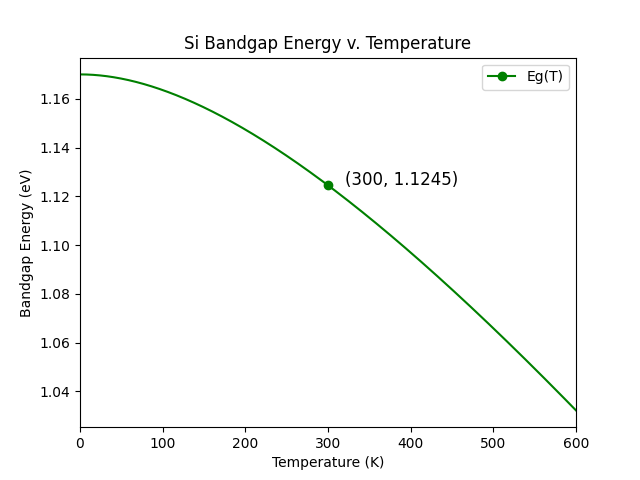
\includegraphics[width = 10cm]{bandgapTempPlot.png}
    \caption{\(E_G\) versus \(T\)}
    \label{fig:bandgapTemp}
\end{figure}

\bigskip

For \(T = 300K\), we see that the bangap energy of Silicon is 1.1245 eV, which is the textbook bandgap for Silicon at room temperature.

\end{document}
